\documentclass{SKP-beamer}

% --------------------------------------------------- %
%                  Presentation info	              %
% --------------------------------------------------- %
\title[General Disease Prediction System]{Predicting the Unpredictable: A General Disease Forecasting System}
\subtitle{Ideation}
\author{Silicon Institute of Technology}
\institute[SBP]{
  DEPARTMENT OF COMPUTER SCIENCE AND ENGINEERING
}
\date{\today}
\logo{
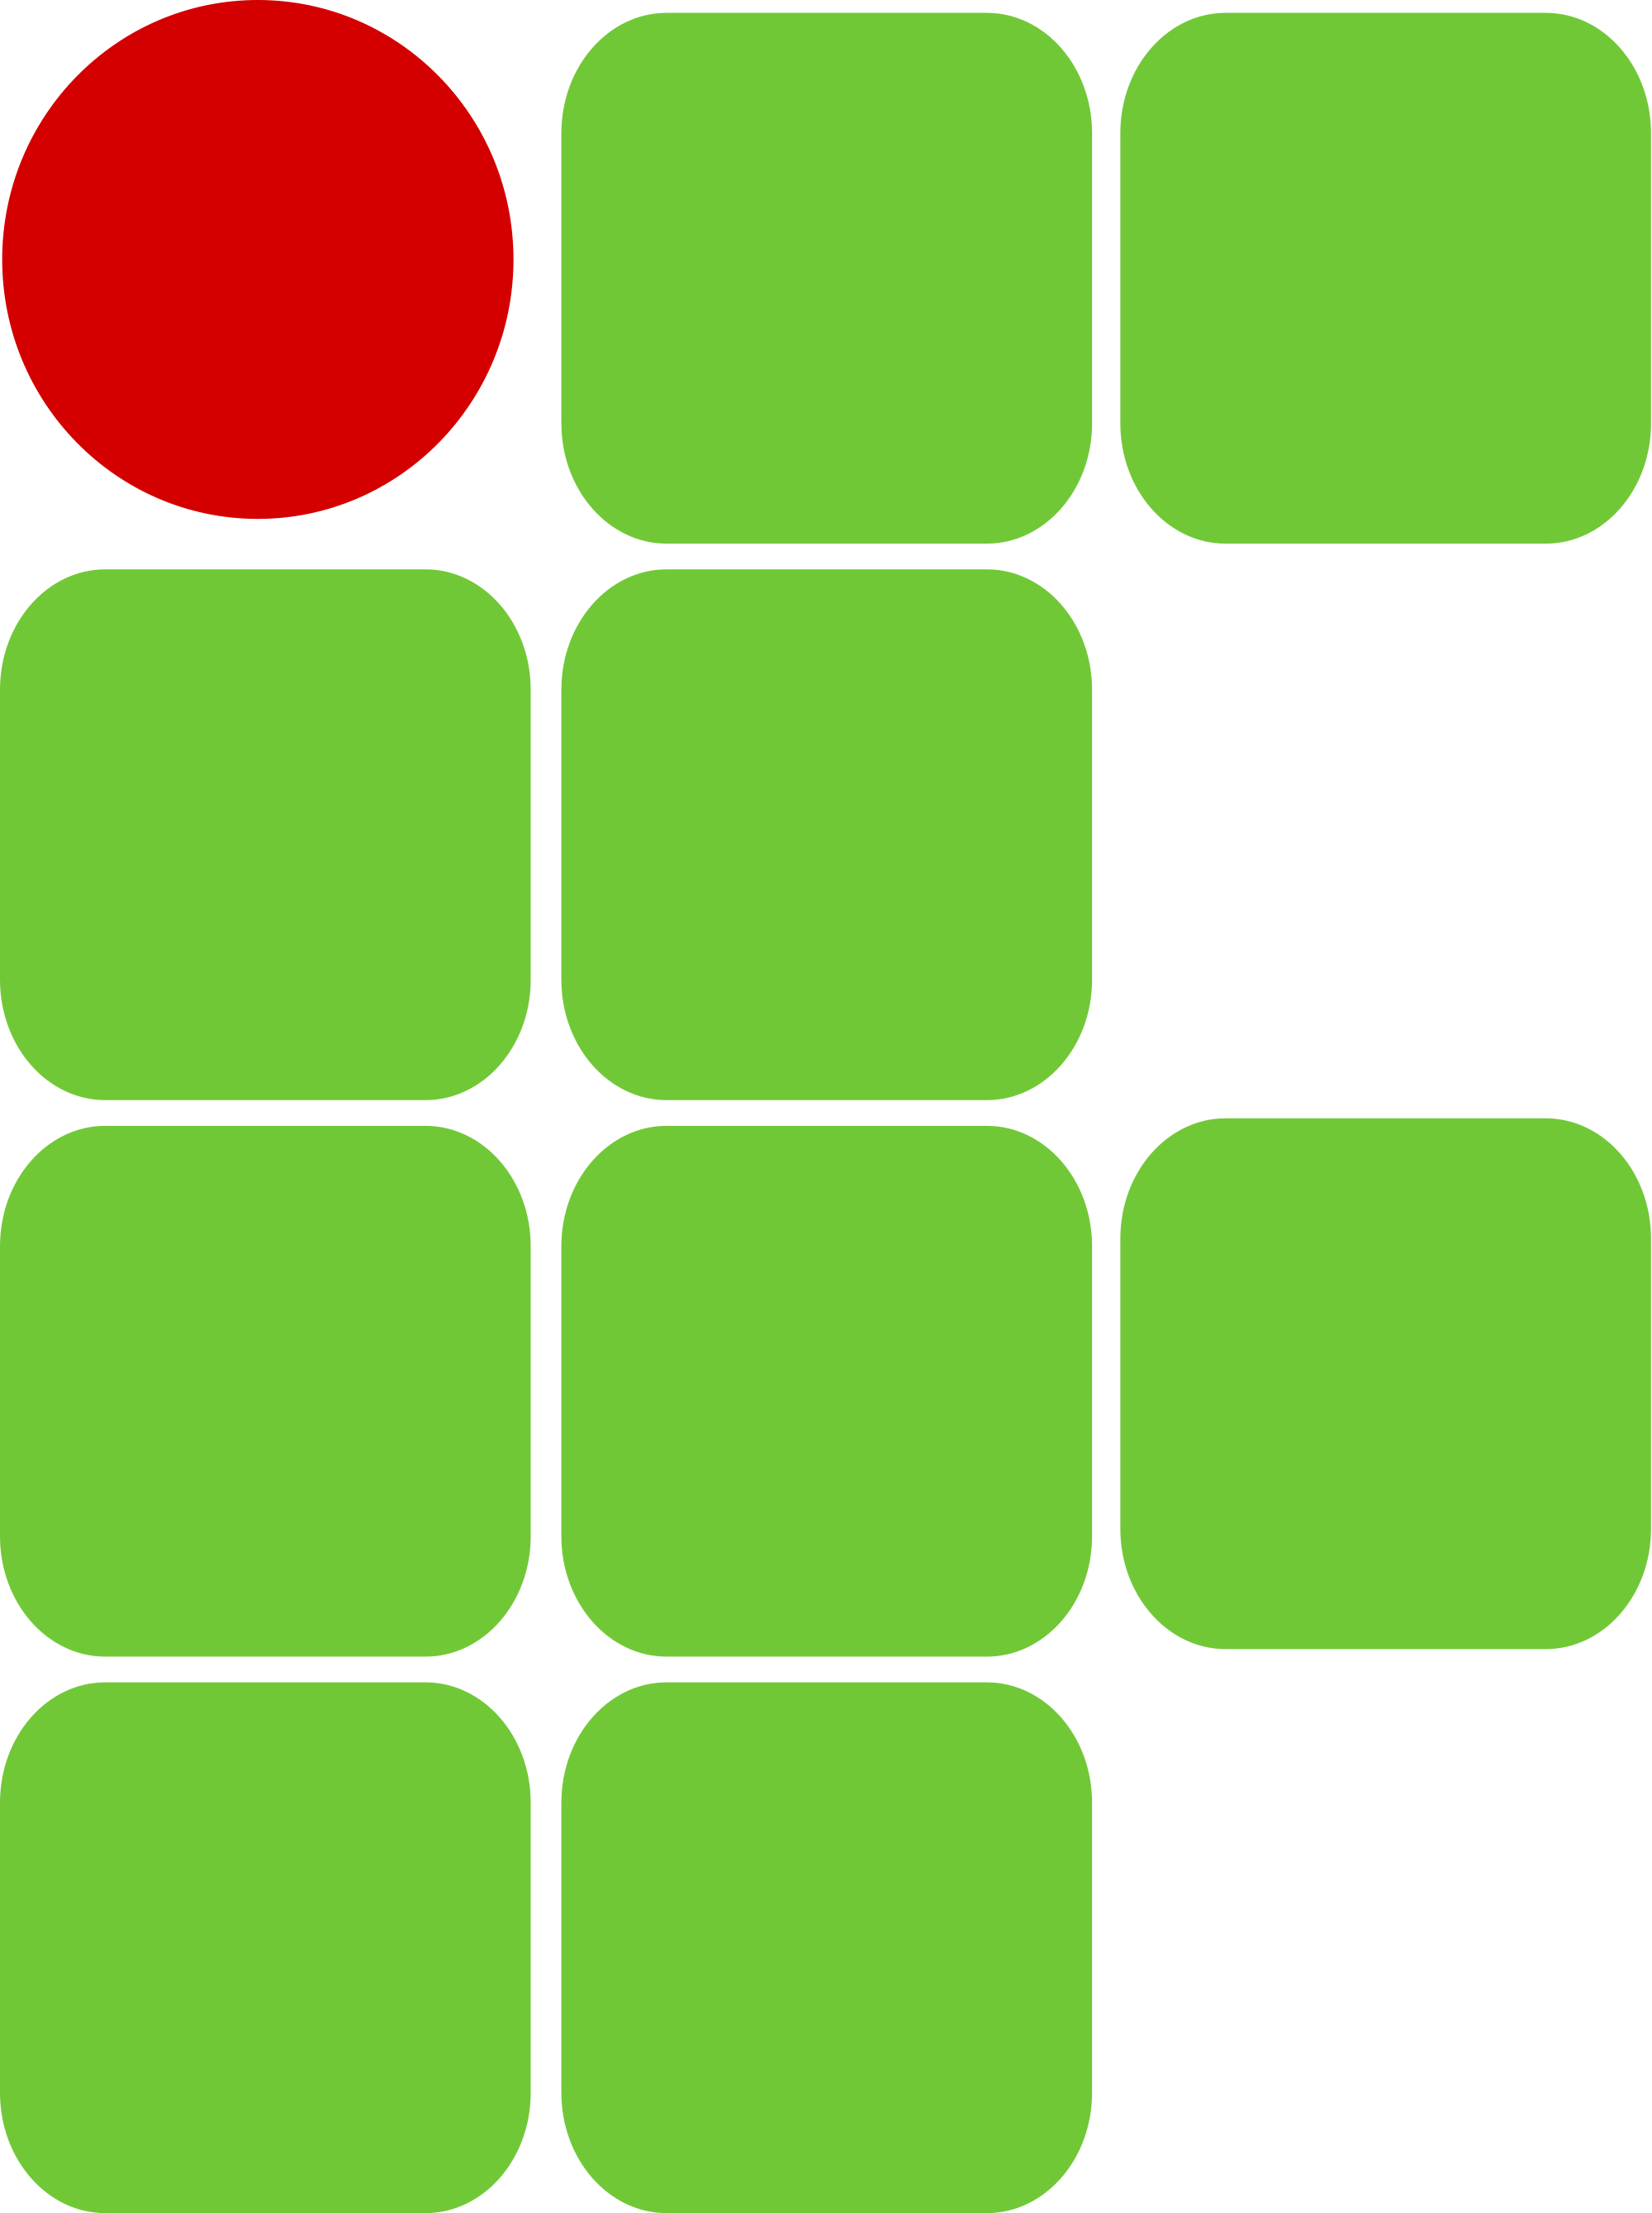
\includegraphics[scale=0.008]{images/logo.png}
}
\subject{Presentation subject} % metadata

% --------------------------------------------------- %
%                    Title + Schedule                 %
% --------------------------------------------------- %

\begin{document}

\begin{frame}
  \titlepage
\end{frame}


\begin{frame}{Table of Contents}
	\begin{itemize}
		\item Introduction
		\item How it Works
		\item Types
		\item Diabetes Prediction System
		\item Heart Disease Prediction System
		\item Breast Cancer Prediction System
		\item Lung Cancer Prediction System
		\item Benefits
		\item Challenges
		\item Future Developments
		\item Conclusion
	\end{itemize}
\end{frame}

\begin{frame}{Motivation}
	\begin{itemize}
		\item Most hospitals today employ some sort of hospital information systems to manage their healthcare or patient data. 
		\item These systems typically generate huge amounts of data which take the form of numbers,text, charts and images. 
		\item Unfortunately, these data are rarely used to support clinical decision making. There is a wealth of hidden information in these data that is largely untapped. This raises an important question:
	   “How can we turn data into useful information that can
	   enable healthcare practitioners to make intelligent
	   clinical decisions?” This is the main motivation for this
	research
\end{itemize}
\end{frame}

\begin{frame}{Introduction}
  The General Disease Prediction System is an innovative technology that uses advanced artificial intelligence algorithms to predict the occurrence of diseases in individuals.
  
  This system is designed to analyze various factors such as age, medical history, lifestyle habits, and environmental conditions to provide accurate predictions
\end{frame}



% --------------------------------------------------- %
%                      Presentation                   %
% --------------------------------------------------- %



\begin{frame}{How it Works}
		The General Disease Prediction System works by collecting and analyzing large amounts of data from various sources such as medical records, genetic testing, and environmental sensors.
		The system then uses machine learning algorithms to identify patterns and correlations between different variables to accurately predict the likelihood of developing certain diseases.
\end{frame}

\section{General Disease Prediction System}

\begin{frame}{General Disease Prediction System}
	\begin{itemize}
	\item Artificial Intelligence made computer more intelligent and can
	enable the computer to think. 
	\item AI study consider machine learning as subfield in numerous research work. Different
	analysts feel that without learning, insight can't be created.
	\item There are numerous kinds of Machine Learning Techniques
	like Unsupervised, Semi Supervised, Supervised,Reinforcement, Evolutionary Learning and Deep Learning.
	\item These learnings are used to classify huge data very fastly. So
	we use K-Nearest Neighbor (KNN) and Convolutional neural
	network (CNN) machine learning algorithm for fast
	classification of big data and accurate prediction of disease.
	\item Because medical data is increasing day by day so usage of that
	for predicting correct disease is crucial task but processing big
	data is very crucial in general so data mining plays very
	important role and classification of large dataset using
	machine learning becomes so easy.
\end{itemize}
\end{frame}

\begin{frame}{System Architecture}
	\begin{center}
	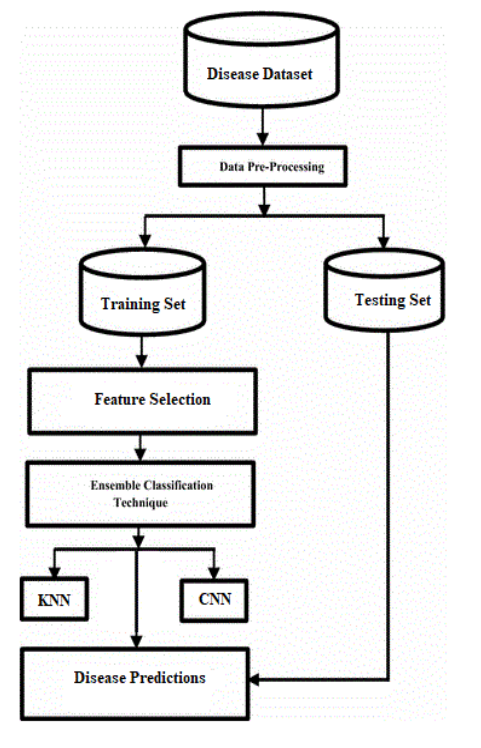
\includegraphics[scale=0.48]{1.png}
\end{center}
\end{frame}

\section{\textbf{Types}}

\begin{frame}{Types of Prediction System}
	\begin{itemize}
		\item Diabetes Prediction System
		\item Lung Cancer Prediction System
		\item Heart Disease Prediction System	
		\item Breast Cancer Prediction System		
	\end{itemize}
\end{frame}



\section{\textbf{Diabetes Prediction System}}

\begin{frame}{Diabetes Prediction System}
	\begin{itemize}
		\item Diabetes is one of deadliest diseases in the
		world. It is not only a disease but also a creator of
		different kinds of diseases like heart attack,
		blindness, kidney diseases, etc.Diabetes Mellitus is defined as a group of metabolic
		disorders mainly caused by abnormal insulin
		secretion and/or action. Insulin deficiency results in
		elevated blood glucose levels (hyperglycemia) and
		impaired metabolism of carbohydrates, fat and
		proteins.
		\item There are two major clinical types : \\ 
		--Type 1 diabetes (T1D) \\
		--Type 2 diabetes (T2D) 
		\item According to the etiopathology
		of the disorder. T2D appears to be the most common
		form of diabetes,mainly characterized by insulin resistance. 
		\item The main causes of T2D include lifestyle, physical activity,dietary habits and heredity, whereas T1D is thought to be due to autoimmunological destruction of the Langerhans islets hosting pancreatic beta cells.	
	\end{itemize}
\end{frame}

\begin{frame}{Working Principle}
	\begin{itemize}
		\item Machine learning is the scientific field
		dealing with the ways in which machines learn from
		experience.The purpose of
		machine learning is the construction of computer
		systems that can adapt and learn from their experiences.
		\item We have developed a system using data
		mining which has the ability to predict whether the
		patient has diabetes or not.
		\item Furthermore, predicting
		the disease early leads to treating the patients before
		it becomes critical. Data mining has the ability to
		extract hidden knowledge from a huge amount of
		diabetes-related data.
		\item The aim of this research is to develop a system
		which can predict the diabetic risk level of a patient
		with a higher accuracy. This research has focused on
		developing a system based on three classification
		methods namely, Support Vector Machine, Logistic
		regression and Artificial Neural Network algorithms. 
	\end{itemize}
\end{frame}

\section{\textbf{Lung Cancer Prediction System}}

\begin{frame}{Lung Cancer Prediction System}
\begin{itemize}
	\item Lung cancer is a harmful disease that causes a huge number of
	deaths globally. 
	\item The primal encounter of lung cancer is necessary to decrease the mortality rate of patients. Thus it is a great challenge encountered by doctors and researchers to
	detect and diagnose lung cancer. 
	\item Detection of lung cancer can be done by using medical images such as computed tomography, chest X-ray; MRI scans, etc., ML approaches recognize the main characteristics of complex lung cancer
	datasets. 
	\item A CAD (Computer-Aided Diagnosis) was developed in the early 1980s to enhance the survival rate and efficiency that aid the doctors in interpreting medical images. 
	\item Some of the machine learning algorithms that have a profound impact in health care are decision trees, linear regression, random forest,SVM, naive Bayes, K-nearest neighbors and so on.
\end{itemize}
\end{frame}


\begin{frame}{Working Principle}
	\begin{itemize}
		\item A prototype lung cancer disease prediction system is
		developed using data mining classification techniques. 
		\item The system extracts hidden knowledge from a historical lung
		cancer disease database. 
		\item The most effective model to predict patients with Lung cancer disease appears to be
		Naïve Bayes followed by IF-THEN rule, Decision Trees and Neural Network.
		\item Decision Trees results are easier to read and interpret. 
		\item The drill through feature to access detailed patients’ profiles is only available in Decision Trees	
	\end{itemize}
\end{frame}

\section{\textbf{Heart Disease Prediction System}}

\begin{frame}{Heart Disease Prediction System}
	\begin{itemize}
		\item Heart disease, alternatively known as cardiovascular disease, encases various conditions that impact the heart and is the primary basis of death worldwide over the span of the past few decades.
		\item  It associates many risk factors in heart disease and a need of the time to get accurate, reliable, and sensible approaches to make an early diagnosis to achieve prompt management of the disease. 
		\item Data mining is a commonly used technique for processing enormous data in the healthcare domain. Researchers apply several data mining and machine learning techniques to analyse huge complex medical data, helping healthcare professionals to predict heart disease. 
		\item This project will be presenting various attributes related to heart disease, and the model on basis of supervised learning algorithms as Naïve Bayes, decision tree, K-nearest neighbor, and random forest algorithm.
	\end{itemize}
\end{frame}

\begin{frame}{Working Principle}
	\begin{itemize}
		\item For predicting heart attack, significantly 15 attributes are listed
		and with basic data mining technique other approaches e.g. ANN,Time Series, Clustering and Association Rules, soft computing approaches etc. can also be incorporated. 
		\item The outcome of predictive data mining technique on the same dataset reveals that
		Decision Tree outperforms and some time Bayesian classification is having similar accuracy as of decision tree but other predictive methods like KNN, Neural Networks, Classification based on clustering are not performing well.
		\item Decision Tree and Bayesian Classification further improves after applying genetic algorithm to reduce the actual data size to get the optimal subset of attribute sufficient for heart disease prediction.
	\end{itemize}
\end{frame}

\section{\textbf{Breast Cancer Prediction System}}

\begin{frame}{Breast Cancer Prediction System}
	\begin{itemize}
		\item Most common type of medical hazard found in middle aged women is, breast cancer. Mortality rate of women due
		to breast cancer can be reduced if can be detected at a relatively early stage.
		\item With the help of latest, efficient and
		advanced screening methods, the majority of such cancers are diagnosed when the disease is still at a localized stage
		\item The utility of machine learning techniques in healthcare analysis is growing progressively. Certainly analysis of patient’s clinical data are the most considerable features in diagnosis. Most of the possible medical flaws can be avoided by the using classification systems
		\item Accurate and timely prediction of breast cancer allows physicians and
		healthcare providers to make most favorable decision about the patient treatment
	\end{itemize}
\end{frame}

\begin{frame}{Proposed Framework}
	    A classification model is proposed with boosted accuracy to predict the breast cancer patient. The framework is composed of the following important phases:
		\begin{itemize}
		\item Dataset Selection
		\item Data Preprocessing
		\item Learning by Classifier (Training) i.e. SVM, Linear Regression and KNN.
		\item Achieving trained model with highest accuracy
		\item Using trained model for prediction
	\end{itemize}
\end{frame}

\begin{frame}{Training and Classification}
	\begin{itemize}
		\item Classifications of the data sets are done on the basis of specific properties posses by the sample variable that the capable to classify them, and each sample variable is assigned a malignant or benign class.
		\item Classification is principally done by making predictions based on known sample data that has been learned from training data. 
		\item Designed algorithm is first trained on the known data labels and further uses this learning to predict the class labels for the new unknown set of data sample
		\item The classification objective set for this study is to achieve enhanced accuracy by using LR, SVM and KNN classifiers and determine which one suits the most for diabetes classification technique
	\end{itemize}
\end{frame}


\begin{frame}{K-Neighbors Classifier Pseudo code}
	\begin{center}
		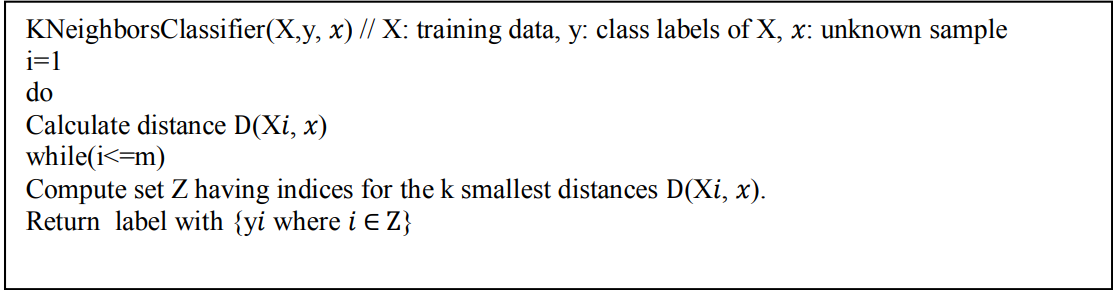
\includegraphics[scale=0.48]{2.png}
	\end{center}
\end{frame}

\section{\textbf{Features}}

\begin{frame}{Features}
	\begin{itemize}
		\item The general disease prediction system is equipped with various features that enable it to accurately predict the spread of diseases. 
		\item One of the primary features of the system is its ability to analyze large amounts of data in real-time. 
		\item This allows it to identify patterns and trends that can be used to predict future outbreaks of diseases. 
		\item Another feature of the system is its ability to integrate with other healthcare systems, such as electronic health records and hospital information systems. This enables it to access a patient's medical history and genetic makeup, which can be used to predict their likelihood of developing certain diseases.
		\item In addition to these features, the general disease prediction system also has a user-friendly interface that makes it easy for healthcare professionals to use. 
		\item The system provides visualizations and dashboards that allow users to quickly and easily interpret complex data. 
		\item It also has built-in analytics tools that enable users to conduct further analysis and refine their predictions over time.
		
	\end{itemize}
\end{frame}

\section{\textbf{Applications}}

\begin{frame}{Applications}
	\begin{itemize}
		\item The general disease prediction system has a wide range of applications in the healthcare industry. One of the primary applications is in disease surveillance, where it can be used to monitor and track the spread of infectious diseases. The system can also be used to predict outbreaks of diseases based on historical data and current trends.
		\item Another application of the system is in personalized medicine. By analyzing a patient's genetic makeup and medical history, the system can predict their likelihood of developing certain diseases and recommend personalized treatment plans. This can lead to better patient outcomes and more effective use of healthcare resources.
	\end{itemize}
\end{frame}


\section{\textbf{Future Developments}}

\begin{frame}{Future Developments}
	\begin{itemize}
	\item As technology continues to advance, the General Disease Prediction System will likely become even more accurate and effective.
	\item New developments in wearable devices, genetic testing, and artificial intelligence will enable the system to provide even more personalized and precise prediction
    \end{itemize}
\end{frame}

\section{\textbf{Conclusion}}

\begin{frame}{Conclusion}
	\begin{itemize}
	\item The General Disease Prediction System represents a major breakthrough in the field healthcare, offering numerous benefits for patients and healthcare providers alike.
	\item While there are still challenges to be addressed, the potential impact of this technology on disease prevention and treatment is immense
    \end{itemize}
\end{frame}

\section{\textbf{References}}

\begin{frame}{References}
	\begin{itemize}
	\item General Disease Prediction System: https://sci-hub.se/10.1109/iccmc.2019.8819782
	\item Diabetes Prediction System : https://sci-hub.se/10.1007/978-3-319-41561-131
	\item Lung Cancer Prediction System : https://sci-hub.se/10.1109/icimia48430.2020.9074947
	\item Breast Cancer Prediction System : https://sci-hub.se/10.1016/j.procs.2018.05.197
	\item Heart Disease Prediction System : https://sci-hub.se/10.1109/aiccsa.2008.4493524
    \end{itemize}	 
\end{frame}

\end{document}
